\section{Chosen Design and Development Process}
%Har gått igenom planeringsrapporten lite noggrannare idag och ser två saker som vi kanske ska borde fånga upp under arbetets gång.

% Under 2 Purpose står det ett upplevelsemål från Young Drive. Bör vi mäta detta upplevelsemål om det stämmer med deltagarnas faktiska upplevelse, d v s ska vi försöka få in det under 3 Research Questions?

% På våra avstämningsmöten borde vi också följa upp dina Research Questions så att kundinteraktionerna och servicedesignmetoden tyligt leder dig framåt mot dessa mål.
%* Reflektioner på vilka designprinciper som bör väljas? (utifrån kundinteraktioner)
%* Reflektioner angående tekniska begränsningar?
%* Reflektioner på processen?

I'm the computer expert kind of designer, but aspiring to be a socio-technical expert (which e.g. Expedition Modial are, as service design experts).

Expedition Mondial will help with a method for creating a MVP of the digital support for the coaches, so that the app is developed from the perspective of the end users and the education and a "learning by doing" mentality. The suggested design process was designed with them after a start-up meeting on Skype, and an Education day in Stockholm. During that day a crash course in service design was given, then creating a common plan for the future work based on my needs.

The result is that the design and development phase in Uganda is an iterative process with the human in focus. The process is built on top of service design process and methodology. There are three iterations.

Expedition Mondial will give support in each iteration, helping with the design of each iteration, and the are able to educate me and assists with the different stages and methodologies. They will assist with recommendations on service design literature, and can highlight reports, previous studies, etc.

Each Interactions phase consists of meeting with two coach groups (one with the app and one without the app), to be able to compare the two and measure effectiveness for research question \#2.

Lena Tibell's and Konrad Schönborn's  competence is extremely valuable to me when formulating questionnaires. How to frame the questions is an art.  Therefore in preparation for meetings with the target group we should discuss exactly what I want to know and they will help to phrase the questions. Then, Expedition Mondial can examine the questions from their a development setting.

The trigger material is used in the Interactions phase of the new iteration. This process you can loop as many times as possible, but the Master Thesis is divided into three iterations.

\begin{figure}[h]
    \centering
    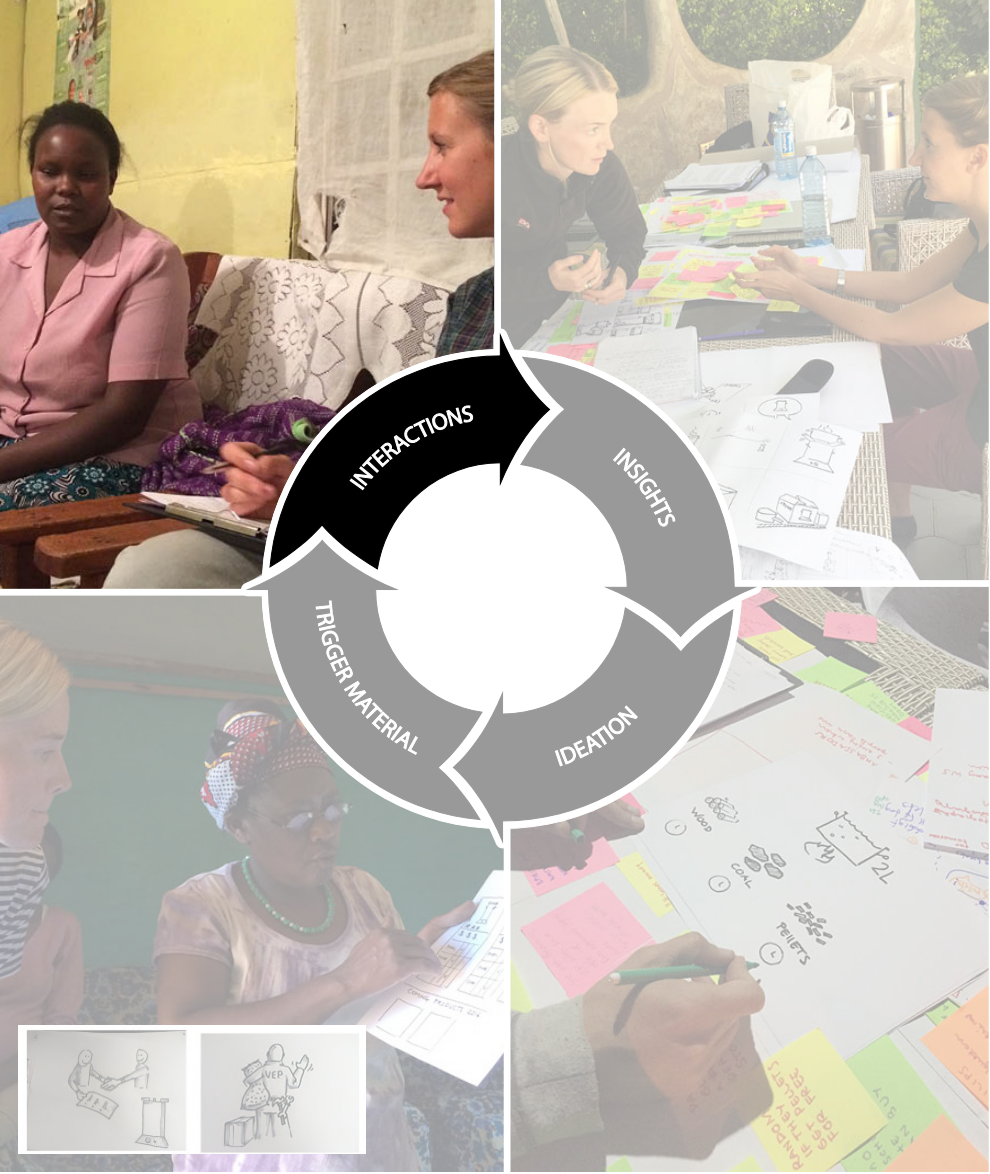
\includegraphics[width=0.7\textwidth]{Iteration.png}
    \caption{One iteration consists of Interactions, Insights, Ideation and Trigger material. The \textbf{Didactic phase} in this figure involves Insights, Ideation and Trigger material. By learning what works and not, new ideas emerge and app design is made, as well as questionnaires for evaluation. The \textbf{Technical phase} in this figure involves to code the improved app design, and evaluate how it works technically.}
    \label{fig:iteration}
\end{figure}

Each iteration ends with two check-up meetings. The first meeting is with the Experts. The next meeting is with the Partners.

The Expert group consists of Expedition Mondial and LiU Innovation. In Expert meetings, I share with them my needs. Expedition Mondial can help with the design process, and LiU Innovation can help if additional resources are needed. The meeting lasts for one hour.

The Partner group consists of most notably Iliana Björling, and preferably also Lena Tibell and Konrad Schönborn. In Partner meetings, The Analysis for the iteration is presented and discussed. Then I will propose possible decisions and discuss the alternatives. % Then I tell them about which decisions has been taken and why.
Finally, we conclude if the master thesis work is going in the right direction. These meetings should be causual and friendly, and not take a lot of time to prepare, so the next iteration can be of focus. % "Kan vara ganska vänskapligt, håll det så enkelt som möjligt så jag får tid till annat."

The time plan for the design and development phase can be seen in the section "In Uganda". The three iterations is presented below: \\

\textbf{The iterations} \\
This is how I want the process to continue:\\

	\textit{\textbf{Iteration 1}}\\
    The first iteration will have a very broad scope. The focus is on the coaches' needs, motivations, and context.  After creation of questions for questionnaire 1, I'll do interviews with coaches and other involved parties. If coaches are met in-group, open questions and dialogue will be done in group for them to be comfortable, posting anonymous answers via post-its on the wall, which leads to specific questions. These sessions will be recorded.

    %resultat: design proposal, Thoughful Interaction Design. "This is where the designer gets involved in design work, establishes a preliminary understanding of the situation, navigates through available information, and initiates all neccessary relationships with clients, users, decision makers, and so forth. Based on all this, she creates a design proposal.

    A first analysis will be done to determine needs, motivations, and expectations. Then, a summarizing meeting will be held with the expert and the partner group to determine possible ways of going forward. A first trigger/paper material will be created, for iteration 2.\\

   \textit{\textbf{Iteration 2}}\\
   This time, the iteration has a more detailed scope, with a hypothesis on what needs the app should meet and in the end, and test the trigger material created to meet those needs.

   I'll be helped with questionnaire material 2. I'll facilitate co-creating interviews with coaches, make an analysis to identify important functionality, and have a summarizing meeting with experts and partners to determine the way forward. A second trigger material will be created, one which was digital, and one which was only made on paper.\\

   \textit{\textbf{Iteration 3}}\\
   Finally, I will be supported with the third iteration, with an even more detailed scope. A co-creation workshop will be held.

   Before the workshop, the wished functionality and goals should be well formulated. Then, it can be discussed how to best design the workshop, together with Lena, Konrad, and Expedition Mondial.

   Questionnaire 3 will be created. In conjunction with the workshop the coaches can be tested, interviewed, and their interactions studied.

In the end of iteration 3, a final analysis will be done, and a final summarizing meeting with experts and partners will determine they way forward.\\
